% Tiêu đề trang dóng theo cột nội dung chính
\noindent
\begin{minipage}[b]{145pt}
~
\end{minipage}\hspace{20.6pt}%
\begin{minipage}[b]{360pt}
\textsf{\textbf{MỤC 4.2}}\quad \textsf{Định lý giá trị trung bình}\hfill \textsf{\textbf{291}}
\vspace{2pt}
\end{minipage}

\vspace{10pt}

\setcolumnwidth{145pt, 360pt}
\setlength{\columnsep}{20.6pt}

\begin{paracol}{2}

% Cột lề trái: Biểu tượng giải quyết vấn đề (PS)
\switchcolumn[0]
\noindent
\tikz[baseline=(X.base)]{%
  \node[fill=pspurple, text=white, font=\bfseries\sffamily\footnotesize, inner sep=2.5pt, rounded corners=1pt] (X) {PS};%
}\hspace{6pt}{\sffamily\bfseries\color{pspurple}\footnotesize Xét các trường hợp}

% Cột chính: Tiếp tục chứng minh Định lý Rolle & Ví dụ 1
\switchcolumn[1]
\noindent{\color{boxred}\textsf{\textbf{CHỨNG MINH}}}\quad Có ba trường hợp:

\smallskip
\noindent\textsf{\textbf{TRƯỜNG HỢP I}}\quad $f(x) = k$, một hằng số. Khi đó $f'(x) = 0$, do đó số $c$ có thể chọn là \textit{bất kỳ} số nào trong khoảng $(a, b)$.

\smallskip
\noindent\textsf{\textbf{TRƯỜNG HỢP II}}\quad $f(x) > f(a)$ với một số $x$ nào đó trong $(a, b)$ \quad \textsf{\small[như trong Hình 1(b) hoặc (c)]}\\
Theo Định lý giá trị cực biên (mà ta có thể áp dụng theo giả thiết 1), $f$ đạt giá trị lớn nhất tại một điểm nào đó trong $[a, b]$. Vì $f(a) = f(b)$ nên nó phải đạt giá trị lớn nhất này tại một số $c$ trong khoảng mở $(a, b)$. Khi đó $f$ có một cực đại \textit{địa phương} tại $c$ và, theo giả thiết 2, $f$ khả vi tại $c$. Do đó $f'(c) = 0$ theo Định lý Fermat.

\smallskip
\noindent\textsf{\textbf{TRƯỜNG HỢP III}}\quad $f(x) < f(a)$ với một số $x$ nào đó trong $(a, b)$ \quad \textsf{\small[như trong Hình 1(c) hoặc (d)]}\\
Theo Định lý giá trị cực biên, $f$ đạt giá trị nhỏ nhất trong $[a, b]$ và, vì $f(a) = f(b)$, nó đạt giá trị nhỏ nhất này tại một số $c$ trong khoảng $(a, b)$. Một lần nữa, $f'(c) = 0$ theo Định lý Fermat.\hfill\textcolor{boxred}{\rule{1.1ex}{1.1ex}}

\bigskip
\noindent{\color{stewartblue}\textsf{\textbf{VÍ DỤ 1}}}\quad Hãy áp dụng Định lý Rolle cho hàm vị trí $s = f(t)$ của một vật chuyển động. Nếu vật ở cùng một vị trí tại hai thời điểm khác nhau $t = a$ và $t = b$, thì $f(a) = f(b)$. Định lý Rolle khẳng định rằng có một thời điểm $t = c$ nào đó giữa $a$ và $b$ sao cho $f'(c) = 0$; nghĩa là vận tốc bằng 0. (Đặc biệt, bạn có thể thấy điều này đúng khi một quả bóng được ném thẳng đứng lên trên).\hfill\textcolor{stewartblue}{\rule{1.1ex}{1.1ex}}

% Dóng hàng chính xác giữa Ví dụ 2 và Hình 2 ở lề
\switchcolumn[0]*

% Cột lề: Ghi chú Hình 2 và Đồ thị
\noindent{\footnotesize\sffamily Hình 2 biểu diễn đồ thị của hàm số $f(x) = x^3 + x - 1$ được thảo luận trong Ví dụ 2. Định lý Rolle cho thấy rằng, cho dù ta có mở rộng khung hình chữ nhật quan sát bao nhiêu đi nữa, ta cũng không bao giờ có thể tìm thấy giao điểm thứ hai với trục $x$.\par}

\vspace{6pt}
\noindent
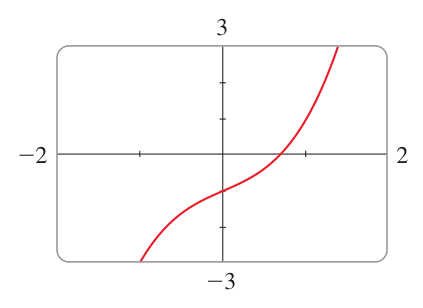
\includegraphics[width=\linewidth]{images/p0326_fig1.png}

\vspace{2pt}
\noindent{\footnotesize\sffamily\textbf{HÌNH 2}}

% Cột chính: Ví dụ 2 và Lời giải
\switchcolumn[1]
\noindent{\color{stewartblue}\textsf{\textbf{VÍ DỤ 2}}}\quad Chứng minh rằng phương trình $x^3 + x - 1 = 0$ có đúng một nghiệm thực.

\smallskip
\noindent{\color{stewartblue}\textsf{\textbf{LỜI GIẢI}}}\quad Trước hết ta dùng Định lý giá trị trung gian (2.5.10) để chỉ ra rằng tồn tại một nghiệm. Đặt $f(x) = x^3 + x - 1$. Khi đó $f(0) = -1 < 0$ và $f(1) = 1 > 0$. Vì $f$ là hàm đa thức nên nó liên tục, do đó Định lý giá trị trung gian khẳng định rằng tồn tại một số $c$ nằm giữa 0 và 1 sao cho $f(c) = 0$. Như vậy phương trình đã cho có nghiệm.

Để chỉ ra rằng phương trình không có nghiệm thực nào khác, ta dùng Định lý Rolle và lập luận bằng phản chứng. Giả sử phương trình có hai nghiệm $a$ và $b$. Khi đó $f(a) = 0 = f(b)$ và, vì $f$ là đa thức nên nó khả vi trên $(a, b)$ và liên tục trên $[a, b]$. Do đó, theo Định lý Rolle, tồn tại một số $c$ nằm giữa $a$ và $b$ sao cho $f'(c) = 0$. Nhưng
\[
  f'(x) = 3x^2 + 1 \ge 1 \qquad \text{với mọi } x
\]
(vì $x^2 \ge 0$) nên $f'(x)$ không bao giờ có thể bằng 0. Điều này mang lại một mâu thuẫn. Vì vậy phương trình không thể có hai nghiệm thực.\hfill\textcolor{stewartblue}{\rule{1.1ex}{1.1ex}}

% Dóng hàng chính xác phần Định lý giá trị trung bình
\switchcolumn[1]*

% Cột chính: Tiêu đề Mục và Khung định lý
\vspace{6pt}
\noindent{\color{stewartblue}\rule{1.2ex}{1.2ex}}\hspace{0.5em}{\large\sffamily\textbf{Định lý giá trị trung bình}}

\smallskip
\noindent Ứng dụng chính của chúng ta về Định lý Rolle là dùng để chứng minh định lý quan trọng sau đây, định lý này lần đầu tiên được phát biểu bởi một nhà toán học Pháp khác, Joseph-Louis Lagrange.

\smallskip
\begin{tcolorbox}[
  enhanced,
  colback=white,
  colframe=boxred,
  arc=0mm,
  boxrule=0.8pt,
  left=8pt, right=8pt, top=6pt, bottom=6pt
]
  \noindent{\sffamily\bfseries\color{boxred}Định lý giá trị trung bình}\quad
  Giả sử $f$ là một hàm số thỏa mãn các giả thiết sau:
  \begin{enumerate}[label=\textbf{\arabic*.}, leftmargin=1.8em, itemsep=1pt, topsep=3pt, parsep=0pt]
    \item $f$ liên tục trên đoạn đóng $[a, b]$.
    \item $f$ khả vi trên khoảng mở $(a, b)$.
  \end{enumerate}
  Khi đó tồn tại một số $c$ trong khoảng $(a, b)$ sao cho
  \vspace{4pt}

  \noindent\makebox[0pt][l]{\redtag{1}}\hfill $\displaystyle f'(c) = \frac{f(b) - f(a)}{b - a}$\hfill\phantom{\redtag{1}}

  \vspace{4pt}
  \noindent hoặc tương đương,
  \vspace{4pt}

  \noindent\makebox[0pt][l]{\redtag{2}}\hfill $\displaystyle f(b) - f(a) = f'(c)(b - a)$\hfill\phantom{\redtag{2}}
\end{tcolorbox}

% Cột lề: Khái niệm Định lý tồn tại dóng ngang khung định lý
\switchcolumn[0]
\vspace{44pt}
\noindent{\footnotesize\sffamily Định lý giá trị trung bình là một ví dụ về cái gọi là \textit{định lý tồn tại}. Tương tự như Định lý giá trị trung gian, Định lý giá trị cực biên và Định lý Rolle, nó đảm bảo rằng \textit{tồn tại} một số có một tính chất nhất định, nhưng nó không chỉ ra cho chúng ta cách tìm ra số đó.\par}

\end{paracol}

\vfill
\begin{center}
{\fontsize{5.5}{7}\selectfont\color{gray!80!black}
Copyright 2021 Cengage Learning. All Rights Reserved. May not be copied, scanned, or duplicated, in whole or in part. WCN 02-200-203\\[1pt]
Editorial review has deemed that any suppressed content does not materially affect the overall learning experience. Cengage Learning reserves the right to remove additional content at any time if subsequent rights restrictions require it.
}
\end{center}
